\section{INSAT-3D Sounder SRFs}
%==============================
\label{app.sndr_srf_data_plots}

\subsection{Channel 1}
\begin{figure}[H]
  \centering
  \begin{tabular}{c}
    \includegraphics[scale=0.55]{graphics/sndr/srf/sndr_insat3d-1.eps} \\
    \includegraphics[scale=0.55]{graphics/sndr/srf/sndr_insat3d-1.difference.eps}
  \end{tabular}
  \caption{INSAT-3D Sounder channel 1 spectral responses. Vertical dashed lines are the locations of the computed central frequencies. \emph{(Top)} Comparison of original and new SRFs. \emph{(Bottom)} Response difference between the original and new SRFs.}
  \label{fig:sndr_ch1}
\end{figure}

\subsection{Channel 2}
\begin{figure}[H]
  \centering
  \begin{tabular}{c}
    \includegraphics[scale=0.55]{graphics/sndr/srf/sndr_insat3d-2.eps} \\
    \includegraphics[scale=0.55]{graphics/sndr/srf/sndr_insat3d-2.difference.eps}
  \end{tabular}
  \caption{INSAT-3D Sounder channel 2 spectral responses. Vertical dashed lines are the locations of the computed central frequencies. \emph{(Top)} Comparison of original and new SRFs. \emph{(Bottom)} Response difference between the original and new SRFs.}
  \label{fig:sndr_ch2}
\end{figure}

\subsection{Channel 3}
\begin{figure}[H]
  \centering
  \begin{tabular}{c}
    \includegraphics[scale=0.55]{graphics/sndr/srf/sndr_insat3d-3.eps} \\
    \includegraphics[scale=0.55]{graphics/sndr/srf/sndr_insat3d-3.difference.eps}
  \end{tabular}
  \caption{INSAT-3D Sounder channel 3 spectral responses. Vertical dashed lines are the locations of the computed central frequencies. \emph{(Top)} Comparison of original and new SRFs. \emph{(Bottom)} Response difference between the original and new SRFs.}
  \label{fig:sndr_ch3}
\end{figure}

\subsection{Channel 4}
\begin{figure}[H]
  \centering
  \begin{tabular}{c}
    \includegraphics[scale=0.55]{graphics/sndr/srf/sndr_insat3d-4.eps} \\
    \includegraphics[scale=0.55]{graphics/sndr/srf/sndr_insat3d-4.difference.eps}
  \end{tabular}
  \caption{INSAT-3D Sounder channel 4 spectral responses. Vertical dashed lines are the locations of the computed central frequencies. \emph{(Top)} Comparison of original and new SRFs. \emph{(Bottom)} Response difference between the original and new SRFs.}
  \label{fig:sndr_ch4}
\end{figure}

\subsection{Channel 5}
\begin{figure}[H]
  \centering
  \begin{tabular}{c}
    \includegraphics[scale=0.55]{graphics/sndr/srf/sndr_insat3d-5.eps} \\
    \includegraphics[scale=0.55]{graphics/sndr/srf/sndr_insat3d-5.difference.eps}
  \end{tabular}
  \caption{INSAT-3D Sounder channel 5 spectral responses. Vertical dashed lines are the locations of the computed central frequencies. \emph{(Top)} Comparison of original and new SRFs. \emph{(Bottom)} Response difference between the original and new SRFs.}
  \label{fig:sndr_ch5}
\end{figure}

\subsection{Channel 6}
\begin{figure}[H]
  \centering
  \begin{tabular}{c}
    \includegraphics[scale=0.55]{graphics/sndr/srf/sndr_insat3d-6.eps} \\
    \includegraphics[scale=0.55]{graphics/sndr/srf/sndr_insat3d-6.difference.eps}
  \end{tabular}
  \caption{INSAT-3D Sounder channel 6 spectral responses. Vertical dashed lines are the locations of the computed central frequencies. \emph{(Top)} Comparison of original and new SRFs. \emph{(Bottom)} Response difference between the original and new SRFs.}
  \label{fig:sndr_ch6}
\end{figure}

\subsection{Channel 7}
\begin{figure}[H]
  \centering
  \begin{tabular}{c}
    \includegraphics[scale=0.55]{graphics/sndr/srf/sndr_insat3d-7.eps} \\
    \includegraphics[scale=0.55]{graphics/sndr/srf/sndr_insat3d-7.difference.eps}
  \end{tabular}
  \caption{INSAT-3D Sounder channel 7 spectral responses. Vertical dashed lines are the locations of the computed central frequencies. \emph{(Top)} Comparison of original and new SRFs. \emph{(Bottom)} Response difference between the original and new SRFs.}
  \label{fig:sndr_ch7}
\end{figure}

\subsection{Channel 8}
\begin{figure}[H]
  \centering
  \begin{tabular}{c}
    \includegraphics[scale=0.55]{graphics/sndr/srf/sndr_insat3d-8.eps} \\
    \includegraphics[scale=0.55]{graphics/sndr/srf/sndr_insat3d-8.difference.eps}
  \end{tabular}
  \caption{INSAT-3D Sounder channel 8 spectral responses. Vertical dashed lines are the locations of the computed central frequencies. \emph{(Top)} Comparison of original and new SRFs. \emph{(Bottom)} Response difference between the original and new SRFs.}
  \label{fig:sndr_ch8}
\end{figure}

\subsection{Channel 9}
\begin{figure}[H]
  \centering
  \begin{tabular}{c}
    \includegraphics[scale=0.55]{graphics/sndr/srf/sndr_insat3d-9.eps} \\
    \includegraphics[scale=0.55]{graphics/sndr/srf/sndr_insat3d-9.difference.eps}
  \end{tabular}
  \caption{INSAT-3D Sounder channel 9 spectral responses. Vertical dashed lines are the locations of the computed central frequencies. \emph{(Top)} Comparison of original and new SRFs. \emph{(Bottom)} Response difference between the original and new SRFs.}
  \label{fig:sndr_ch9}
\end{figure}

\subsection{Channel 10}
\begin{figure}[H]
  \centering
  \begin{tabular}{c}
    \includegraphics[scale=0.55]{graphics/sndr/srf/sndr_insat3d-10.eps} \\
    \includegraphics[scale=0.55]{graphics/sndr/srf/sndr_insat3d-10.difference.eps}
  \end{tabular}
  \caption{INSAT-3D Sounder channel 10 spectral responses. Vertical dashed lines are the locations of the computed central frequencies. \emph{(Top)} Comparison of original and new SRFs. \emph{(Bottom)} Response difference between the original and new SRFs.}
  \label{fig:sndr_ch10}
\end{figure}

\subsection{Channel 11}
\begin{figure}[H]
  \centering
  \begin{tabular}{c}
    \includegraphics[scale=0.55]{graphics/sndr/srf/sndr_insat3d-11.eps} \\
    \includegraphics[scale=0.55]{graphics/sndr/srf/sndr_insat3d-11.difference.eps}
  \end{tabular}
  \caption{INSAT-3D Sounder channel 11 spectral responses. Vertical dashed lines are the locations of the computed central frequencies. \emph{(Top)} Comparison of original and new SRFs. \emph{(Bottom)} Response difference between the original and new SRFs.}
  \label{fig:sndr_ch11}
\end{figure}

\subsection{Channel 12}
\begin{figure}[H]
  \centering
  \begin{tabular}{c}
    \includegraphics[scale=0.55]{graphics/sndr/srf/sndr_insat3d-12.eps} \\
    \includegraphics[scale=0.55]{graphics/sndr/srf/sndr_insat3d-12.difference.eps}
  \end{tabular}
  \caption{INSAT-3D Sounder channel 12 spectral responses. Vertical dashed lines are the locations of the computed central frequencies. \emph{(Top)} Comparison of original and new SRFs. \emph{(Bottom)} Response difference between the original and new SRFs.}
  \label{fig:sndr_ch12}
\end{figure}

\subsection{Channel 13}
\begin{figure}[H]
  \centering
  \begin{tabular}{c}
    \includegraphics[scale=0.55]{graphics/sndr/srf/sndr_insat3d-13.eps} \\
    \includegraphics[scale=0.55]{graphics/sndr/srf/sndr_insat3d-13.difference.eps}
  \end{tabular}
  \caption{INSAT-3D Sounder channel 13 spectral responses. Vertical dashed lines are the locations of the computed central frequencies. \emph{(Top)} Comparison of original and new SRFs. \emph{(Bottom)} Response difference between the original and new SRFs.}
  \label{fig:sndr_ch13}
\end{figure}

\subsection{Channel 14}
\begin{figure}[H]
  \centering
  \begin{tabular}{c}
    \includegraphics[scale=0.55]{graphics/sndr/srf/sndr_insat3d-14.eps} \\
    \includegraphics[scale=0.55]{graphics/sndr/srf/sndr_insat3d-14.difference.eps}
  \end{tabular}
  \caption{INSAT-3D Sounder channel 14 spectral responses. Vertical dashed lines are the locations of the computed central frequencies. \emph{(Top)} Comparison of original and new SRFs. \emph{(Bottom)} Response difference between the original and new SRFs.}
  \label{fig:sndr_ch14}
\end{figure}

\subsection{Channel 15}
\begin{figure}[H]
  \centering
  \begin{tabular}{c}
    \includegraphics[scale=0.55]{graphics/sndr/srf/sndr_insat3d-15.eps} \\
    \includegraphics[scale=0.55]{graphics/sndr/srf/sndr_insat3d-15.difference.eps}
  \end{tabular}
  \caption{INSAT-3D Sounder channel 15 spectral responses. Vertical dashed lines are the locations of the computed central frequencies. \emph{(Top)} Comparison of original and new SRFs. \emph{(Bottom)} Response difference between the original and new SRFs.}
  \label{fig:sndr_ch15}
\end{figure}

\subsection{Channel 16}
\begin{figure}[H]
  \centering
  \begin{tabular}{c}
    \includegraphics[scale=0.55]{graphics/sndr/srf/sndr_insat3d-16.eps} \\
    \includegraphics[scale=0.55]{graphics/sndr/srf/sndr_insat3d-16.difference.eps}
  \end{tabular}
  \caption{INSAT-3D Sounder channel 16 spectral responses. Vertical dashed lines are the locations of the computed central frequencies. \emph{(Top)} Comparison of original and new SRFs. \emph{(Bottom)} Response difference between the original and new SRFs.}
  \label{fig:sndr_ch16}
\end{figure}

\subsection{Channel 17}
\begin{figure}[H]
  \centering
  \begin{tabular}{c}
    \includegraphics[scale=0.55]{graphics/sndr/srf/sndr_insat3d-17.eps} \\
    \includegraphics[scale=0.55]{graphics/sndr/srf/sndr_insat3d-17.difference.eps}
  \end{tabular}
  \caption{INSAT-3D Sounder channel 17 spectral responses. Vertical dashed lines are the locations of the computed central frequencies. \emph{(Top)} Comparison of original and new SRFs. \emph{(Bottom)} Response difference between the original and new SRFs.}
  \label{fig:sndr_ch17}
\end{figure}

\subsection{Channel 18}
\begin{figure}[H]
  \centering
  \begin{tabular}{c}
    \includegraphics[scale=0.55]{graphics/sndr/srf/sndr_insat3d-18.eps} \\
    \includegraphics[scale=0.55]{graphics/sndr/srf/sndr_insat3d-18.difference.eps}
  \end{tabular}
  \caption{INSAT-3D Sounder channel 18 spectral responses. Vertical dashed lines are the locations of the computed central frequencies. \emph{(Top)} Comparison of original and new SRFs. \emph{(Bottom)} Response difference between the original and new SRFs.}
  \label{fig:sndr_ch18}
\end{figure}
